\documentclass{sig-alternate-2013}

% UTF8 support
\usepackage[utf8x]{inputenc}
\usepackage[T1]{fontenc}

\usepackage{graphicx}
\graphicspath{{figs/}}
\usepackage{tikz}
\usetikzlibrary{shapes}

\usepackage{array}

\usepackage{color, soul}

\newcommand{\eg}{{\textit{e.g.~}}}
\newcommand{\etal}{{\textit{et al.~}}}
\newcommand{\ie}{{\textit{i.e.~}}}

\usepackage[nomargin, footnote]{fixme}

\begin{document}

\title{The Cognitive Correlates of Anthropomorphism}

\numberofauthors{2} 
\author{
\alignauthor
Séverin Lemaignan\\
Julia Fink\\
Pierre Dillenbourg\\
    \affaddr{Computer-Human Interaction in\\ Learning and Instruction (CHILI)}\\
    \affaddr{Ecole Polytechnique Fédérale\\ de Lausanne (EPFL)}\\
    \affaddr{CH-1015 Lausanne, Switzerland}\\
    \email{firstname.lastname@epfl.ch}
\alignauthor
Claire Braboszcz\\
    \affaddr{Laboratory for Neurology \& \\Imaging of Cognition (LabNIC)}\\
    \affaddr{University of Geneva}\\
    \affaddr{CH-1211 Geneva, Switzerland}\\
    \email{claire.braboszcz@unige.ch}
}

\maketitle

\begin{abstract}

While anthropomorphism in human-robot interaction is often discussed, it still
appears to lack formal grounds. We recently proposed a first model of the
\emph{dynamics of anthropomorphism} that reflects the
evolution of anthropomorphism in the human-robot interaction over time. The
model also accounts for non-monotonic effects like the so-called \emph{novelty
effect}.

This contribution proposes to build upon this model to investigate the
\emph{cognitive correlates} induced by a sustained human-robot interaction and
we present here our initial ideas. We propose to distinguish three cognitive
phases: \emph{pre-cognitive}, \emph{familiarity}-based, and \emph{adapted}
anthropomorphism, and we outline how these phases relate to the phenomenological
evolution of anthropomorphism over time.

\end{abstract}


\section{Introduction}
\label{sec:intro}

We recently presented a new model of anthropomorphism that focuses on the
dynamics of this phenomenon~\cite{lemaignan2014dynamics}.

Many robotics researchers tend indeed to believe that \emph{anthropomorphism}
describes a static set of human-like features of a robot (like shape, speech
capabilities, facial expression). We refer to these characteristics as the
\emph{anthropomorphic design} of the robot~\cite{fink_anthropomorphism_2012}.
\emph{Anthropomorphism}, on the other hand, refers to the \emph{social
phenomenon} that emerges from the \emph{interaction} between a robot and a
user. According to Epley \etal\cite{epley_when_2008}, this includes for
instance emotional states, motivations, intentions \emph{ascribed by the user}
to the robot. As such, anthropomorphism is fundamentally dynamic.

Based on a literature review which was previously
published~\cite{fink_anthropomorphism_2012}, a long-term field study in a
natural environment~\cite{fink_living_2013}, as well as two on-going child-robot
experiments~\cite{fink2014which}, we believe that \emph{anthropomorphic effects}
(\ie the observable manifestations of anthropomorphism) not only evolve over
time, but that they do so in non-monotonic ways. We show here how they also reflect cognitive
processes experienced by the human peer when interacting with the robot.

In the following sections we first describe our model of the dynamics of
anthropomorphism.  We then adopt a cognitive perspective on anthropomorphism,
and outline how the dynamics of anthropomorphism can be interpreted from this
viewpoint. 


\section{Dynamics of Anthropomorphism}
\label{sec:dynamics_model}

Figure~\ref{fig:dynamics} represents the phenomenological model of the long-term
dynamics of anthropomorphic effects that we call the \emph{dynamics of
anthropomorphism}~\cite{lemaignan2014dynamics}. The model is split into three
phases, depicted in different shades on the figure.

In this model, anthropomorphism is quantified by a \emph{normalized level of
anthropomorphic effects}: because anthropomorphic effects are not quantified on
an absolute scale, we present them as a normalized value, that spans from a
minimum (no anthropomorphic effects) to a maximum (corresponding to the novelty
effect peak on Figure~\ref{fig:dynamics}). The actual maximum value of
anthropomorphic effects depends on each unique combination of human, robot and
several other factors we introduce below, and thus varies. The general
\emph{shape} of the model remains however the same and depicts the evolution of
anthropomorphism over time, \ie the general dynamics of anthropomorphism.

The model takes into account the duration of the interaction, the nature of the
interaction, as well as acquired experience and familiarization mechanisms. We
also formally introduce a so-called \emph{novelty effect} that models the first
phase of human-robot interaction, during which a specific increase of
anthropomorphic interactions is observed. We focus on \emph{long-term
interaction}, \ie direct (non-mediated), repeated interaction with the same
robot, over an extended period of time (typically longer than a week).


\begin{figure*}[htb]
\centering


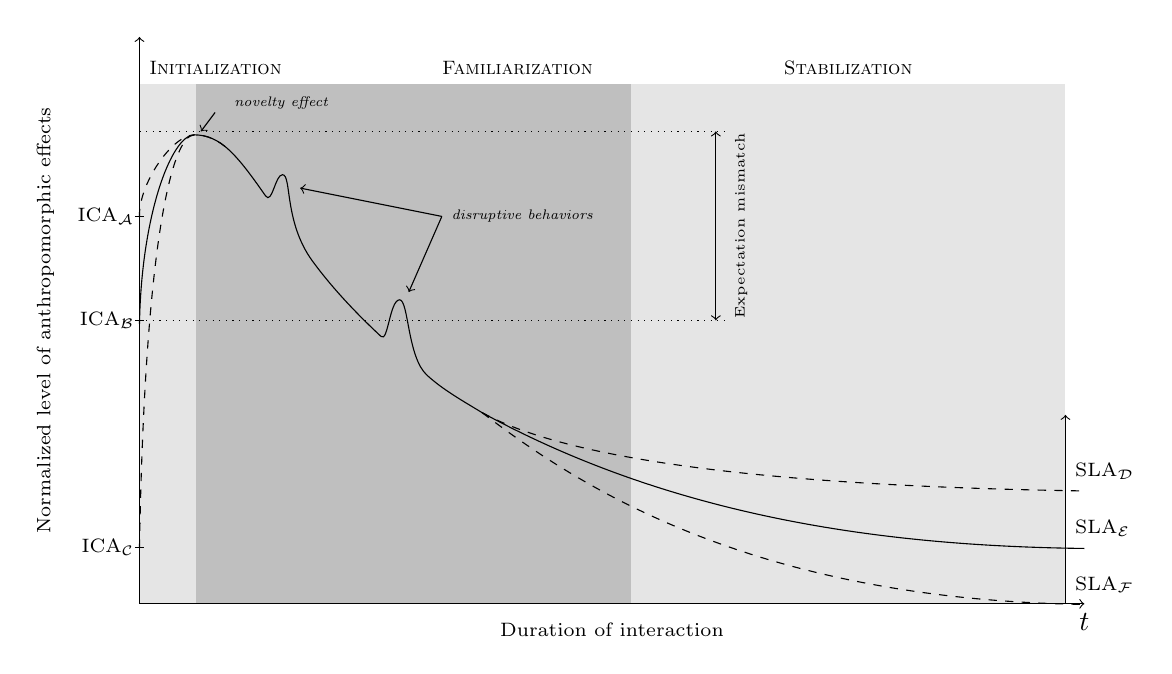
\begin{tikzpicture}[scale=1.2]

% background shading
\path[fill=gray!20] (0,0) rectangle (0.6,5.5);
\path[fill=gray!50] (0.6,0) rectangle (5.2,5.5);
\path[fill=gray!20] (5.2,0) rectangle (9.8,5.5);
\draw(0,5.5) node[anchor=south west] {\scriptsize \sc Initialization};
\draw(4,5.5) node[anchor=south] {\scriptsize \sc Familiarization};
\draw(7.5,5.5) node[anchor=south] {\scriptsize \sc Stabilization};
% horizontal axis
\draw[->] (0,0) -- (10,0) node[anchor=north] {$t$};
\draw(5,-0.1) node[anchor=north] {\scriptsize Duration of interaction};


% vertical axis
\draw[->] (0,0) -- (0,6) node[anchor=east] {};
\draw(-0.8,3) node[rotate=90,anchor=south] {\scriptsize Normalized level of anthropomorphic effects};

\draw (-0.05, 3) -- (0.05, 3) node[anchor=east] {\scriptsize ICA$_{\mathcal B}$};
\draw (-0.05, 4.1) -- (0.05, 4.1) node[anchor=east] {\scriptsize ICA$_{\mathcal A}$};
\draw (-0.05, 0.6) -- (0.05, 0.6) node[anchor=east] {\scriptsize ICA$_{\mathcal C}$};

% vertical axis - end
\draw[->] (9.8,0) -- (9.8,2) node[anchor=east] {};
\draw (9.8, 0.8) node[anchor=west] {\scriptsize SLA$_\mathcal{E}$};
\draw (9.8, 1.4) node[anchor=west] {\scriptsize SLA$_\mathcal{D}$};
\draw (9.8, .2) node[anchor=west] {\scriptsize SLA$_\mathcal{F}$};


\draw[<-] (0.65,5) -- (0.8,5.2) node[anchor=east] {};
\draw (0.9,5.3) node[anchor=west] {\tiny \it novelty effect};


\draw[dotted] (0, 5) -- (6.2,5);
\draw[dotted] (0, 3) -- (6.2,3);
\draw[<->] (6.1,3) -- (6.1,5) node[anchor=east] {};
\draw (6.2,4) node[rotate=90, anchor=north] {\tiny Expectation mismatch};

\draw[<-] (1.7,4.4) -- (3.2,4.1) node[anchor=east] {};
\draw[<-] (2.85,3.3) -- (3.2,4.1) node[anchor=east] {};
\draw (3.2,4.1) node[anchor=west] {\tiny \it disruptive behaviors};
%%%%%
%% CURVES
%%%%
\begin{scope}[yscale=-1,shift={(-0.125,-0.4)}]

% output of inkscape2tikz
\path[draw=black]
    (0.1250,-2.5620) .. controls (0.1451,-3.7193) and (0.4645,-4.5602) ..
    (0.7044,-4.5633) .. controls (0.8413,-4.5633) and (0.9599,-4.5104) ..
    (1.0794,-4.3971) .. controls (1.1989,-4.2841) and (1.3191,-4.1185) ..
    (1.4588,-3.9181) .. controls (1.5287,-3.8183) and (1.5610,-4.1413) ..
    (1.6381,-4.1420) .. controls (1.7378,-4.1420) and (1.6515,-3.6434) ..
    (1.9554,-3.2280) .. controls (2.1466,-2.9667) and (2.3889,-2.7023) ..
    (2.6819,-2.4292) .. controls (2.7551,-2.3607) and (2.7727,-2.8119) ..
    (2.8771,-2.8180) .. controls (2.9742,-2.8180) and (2.9594,-2.2108) ..
    (3.1665,-2.0209) .. controls (3.3340,-1.8673) and (3.5379,-1.7527) ..
    (3.7508,-1.6236) .. controls (5.8366,-0.4852) and (8.0977,-0.2106) ..
    (10.1250,-0.1860);
\path[draw=black, dashed]
    (0.1250,-3.6924) .. controls (0.1103,-4.0298) and (0.4645,-4.5602) .. 
    (0.7044,-4.5633)
    (3.7508,-1.6236) .. controls (4.9579,-0.9555) and (8.1358,-0.8261) .. 
    (10.1250,-0.7946);
\path[draw=black,dashed]
    (0.1250,-0.1953) .. controls (0.1804,-3.3871) and (0.4645,-4.5602) .. 
    (0.7044,-4.5633) .. controls (0.8413,-4.5633) and (0.9599,-4.5104) .. 
    (1.0794,-4.3971)
    (3.7508,-1.6236) .. controls (4.7654,-0.8505) and (6.5955,0.3538) .. 
    (10.1250,0.4062);

\end{scope}

\end{tikzpicture}

\caption{The dynamics of anthropomorphism. We distinguish three main phases:
\emph{initialization}, \emph{familiarization} and \emph{stabilization},
preceded by a \emph{pre-interaction} phase. In the pre-interaction phase,
users build an \emph{initial capital of anthropomorphism} (ICA). Once the
interaction starts, the level of anthropomorphism increases due to the
\emph{novelty effect}, and then decreases to reach a \emph{stabilized level
of anthropomorphism} (SLA).  During the interaction, unpredicted behaviors
of the robot (\emph{disruptive behaviors}) may lead to local increase of the
level of anthropomorphism.}

\label{fig:dynamics}
\end{figure*}

%\subsection*{Three phases}
%\label{sec:phases}

\subsection*{Initialization} During this short phase (which lasts from a couple
of seconds to a couple of hours), an increase of anthropomorphic effects is
observed, from the \emph{initial capital of anthropomorphism} to a peak of
anthropomorphic manifestations that corresponds to the maximum of the
\emph{novelty effect}.

The \emph{initial capital of anthropomorphism} describes the initial potential
for the robot to be anthropomorphized by the human user in a given situation.
This potential depends on several factors. It has been shown, for instance, that
some \textit{people} tend to anthropomorphize more than others, that some
\textit{situations} induce anthropomorphism more than others, that
\textit{children} tend to anthropomorphize more than adults, and that some
\textit{cultures} are notorious for their anthropomorphic religions and
worldviews~\cite{epley_when_2008}. Also the shape and design of the robot play a
role, and the context in which the interaction takes place. Our model of
anthropomorphism takes these determinants into account and initializes the level
of anthropomorphic interactions between a human and a robot to a value that we
call \emph{initial capital of anthropomorphism} (ICA). The ICA describes the
first (real or imagined) contact to a robot. In this stage of pre-interaction,
people form initial expectations toward the robot and imagine how they will use
it / interact with it.

We build the ICA on three main factors that \emph{a priori} determine the
potential that a robot will be anthropomorphized:

\begin{enumerate}

    \item \emph{Human-centered factor}: The \textbf{personality} and individual
        traits of the human user: Psychological characteristics / determinants
        that influence a person's tendency to anthropomorphize
        artifacts~\cite{epley_seeing_2007}. Other individual traits and
        demographic aspects are comprised (\eg age, gender, cultural
        background, professional background).
	
    \item \emph{Robot-centered factor}: The robot's \textbf{design} and how it
        appears to the human user. Characteristics of the robot's form,
        behavior, and interaction modalities (anthropomorphic
        design)~\cite{fong_survey_2003}.
	
    \item \emph{Situation-centered factor}: The real or imagined
        \textbf{purpose} of the robot, including the situational context in
        which it is used, as well as the task context and role in which the robot is 				used / experienced (environmental context)~\cite{joosse_what_2013}.

\end{enumerate}	

By taking the \textbf{purpose} of a robot into account, we suggest that the real
or imagined context in which a robot is used and the interaction that this usage
brings along, impacts how far the robot will be attributed human-like
characteristics. We draw on findings such as presented in Joosse
\etal~\cite{joosse_what_2013}. The authors showed for instance that when the
same robot (NAO) is used in a different task context (cleaning task \emph{vs.}
tour guide), users ascribe different ``personalities'' to the robot. In general,
a robot which is imagined to be used in a social, entertaining or playful
context leads to a higher ICA than a robot which is used for a routine or
focused task (security, rescue, etc.). This idea also receives support from
Goetz \& Kiesler's work that revealed that people prefer a serious robot for
serious tasks and a less serious robot for more playful
tasks~\cite{goetz_cooperation_2002, goetz_matching_2003}. Also, we suggest that
the environmental context in which people experience and interact with the robot
impacts the ICA. For instance, several friends interacting simultaneously with
the robot might lead to increased ICAs, due to increased human-human social
interactions (the robot might be perceived to be part of the social interaction,
and in turn attributed human-like qualities)~\cite{baxter2013do}.

\fxnote{Anything else on Initialization phase?}

\subsection*{Familiarization} The second phase in the dynamics of
anthropomorphism lasts longer (up to several days) and models the process of the
human getting acquainted to the robot: by observation and interaction, the human
builds a model of the robot's behavior that allows him/her to predict the
robot's actions. We observe a decrease of anthropomorphic effects during this
phase, that we explain by the acquired ability to predict the behavior of the
robot: the initial apparent behavioral complexity vanishes, and the robot is
considered more and more as a tool.

\subsection*{Stabilization} The \emph{stabilization} phase spans over a longer
period of time. The level of anthropomorphic effects tends to stabilize, to
reach a \emph{stabilized level of anthropomorphism} (SLA). The SLA may be zero
(no anthropomorphic effects observed anymore), but it may also remain at a
higher level. The \emph{Stabilized Level of Anthropomorphism} describes hence
the long-term lasting, sustained level of anthropomorphism.

We proposed that the ICA is built on three factors: user's \emph{personality},
robot's \emph{design} and interaction \emph{purpose} (or \emph{interaction
context}). The user's personality and the context of use do also influence the
SLA. In particular, it appears that the user's level of acquaintance with
technologies plays an important role in long-term tendency to
anthropomophize~\cite{fink_living_2013} (people more familiar with technology
understand, and hence predict, better the behavior of the robot, which in turn
leads them more frequently to ultimately consider the robot as a simple tool).

The robot's design, on the other hand, plays a more subtle role, and strong
initial anthropomorphic design does not mandate high SLA: lasting
anthropomorphic effects have been observed on non-anthropomorphic robots (like
the iRobot Roomba~\cite{fink_living_2013} or the military iRobot
PackBot\footnote{Rodney Brooks has reported in keynotes that occasionally
soldiers would give a name to \emph{their} PackBot and require it to be repaired
instead of being replaced by another one in case of incident.}), and on the
contrary, anthropomorphic designs can lead to higher expectation deceptions,
resulting in the robot not being used anymore.

Note that the \emph{Initial Capital of Anthropomorphism} and the
\emph{Stabilized Level of Anthropomorphism} are generally not correlated: one
individual may have high potential of anthropomorphizing (high ICA) at first
sight of a good-looking humanoid robot, and get disappointed by the actual
abilities of the robots, down to routine, non-anthropomorphic, interactions
(low SLA), while another user with the same high ICA may, for instance, creates
lasting affective bonds with the same robot, and keeps anthropomorphizing it
(higher SLA).


\section{Cognitive interpretation}
\label{sec:cognitivemodel}

\begin{figure*}[htb]
\centering
%\resizebox{\linewidth}{!}{
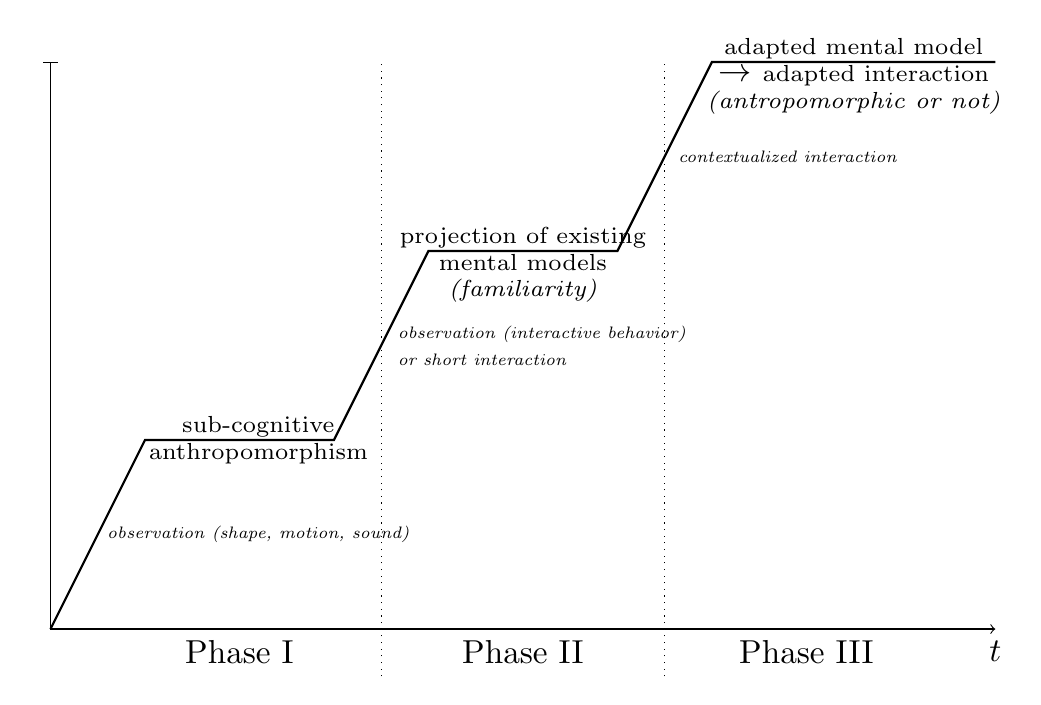
\begin{tikzpicture}[scale=1.2, transform shape]
\baselineskip=8pt

% horizontal axis
\draw[->] (0,0) -- (10,0) node[anchor=north] {$t$};
% labels
\draw   (2,0) node[anchor=north] {Phase I}
        (5,0) node[anchor=north] {Phase II}
        (8,0) node[anchor=north] {Phase III};

\draw[dotted] (3.5, -0.5) -- (3.5,6);
\draw[dotted] (6.5, -0.5) -- (6.5,6);

% vertical axis
\draw[-|] (0,0) -- (0,6) node[anchor=east] {};
% Us
\draw[thick] (0,0) -- (1,2) -- (3,2) -- (4,4) -- (6,4) -- (7,6) -- (10,6);

\draw (2.2,2) node[align=center] {\scriptsize{sub-cognitive}\\\scriptsize{anthropomorphism}}; %label
\draw (5,3.85) node[align=center] {\scriptsize{projection of existing}\\\scriptsize{mental models}\\\scriptsize{\it (familiarity)}}; %label
\draw (8.5,5.85) node[align=center] {\scriptsize{adapted mental model} \\ $\to$ \scriptsize{adapted interaction}\\\scriptsize{\it (antropomorphic or not)}}; %label

\draw (2.2,1) node[align=left] {\tiny{\it observation (shape, motion, sound)}}; %label
\draw (5.2,3) node[align=left] {\tiny \it observation (interactive behavior) \\ \tiny \it or short interaction}; %label
\draw (7.8,5) node[align=left] {\tiny \it contextualized interaction}; %label

\end{tikzpicture}
%}
\caption{The three cognitive phases of anthropomorphism: Phase I is the instinctive,
sub-cognitive identification of living peers. {\it Empathy} is characteristic
of this stage. After longer observation or short, non-contextualized interaction
(typically, a lab environment), the user enters Phase II: the user projects a
mental model he/she is already familiar with onto the robot. After longer {\it
contextualized} interaction (typically, at home), the user enters Phase III of
anthropomorphism: the user recomposes an accurate mental model of the robot,
based on experience. This leads to adapted interaction modalities, that may
still be anthropomorphic, or not.}
\label{fig:cognitivemodel}
\end{figure*}


We provide in this section a tentative interpretation of anthropomorphism in
terms of cognitive correlates. We warmly welcome the feedback and
comments from both the cognitive sciences and robotics communities to further
discuss these findings.

We propose three different cognitive phases (Figure~\ref{fig:cognitivemodel}),
which do not directly match the previously presented three phases of
anthropomorphism but are still related.


\subsection*{Explanations for anthropomorphism}

Anthropomorphism represents just one of many examples of induction whereby
``people reason about an unknown stimulus based on a better-known representation
of a related stimulus"~\cite{epley_when_2008}, in this case reasoning about a
non-human agent based on representation of the self or other humans.

According to Lee \etal~\cite{lee_human_2005}, there are two main perspectives in
explaining people's tendency to anthropomorphize. First one explains
anthropomorphism from the design of the artifact. It assumes that humans
directly respond to life-like or social cues that an object or system emits,
without thoughtful mental processing, by simply applying stereotypes and
heuristics to it. In fact, from early childhood on, humans are inherently
well-trained to perceive life \cite{epley_seeing_2007}. Schmitz
\cite{schmitz_concepts_2011} describes that within the visual scope of design,
the outer appearance can have an important impact on the overall perception of
an object. The basic assumption here is that if an artifact appears much like a
human, it is likely to be treated similar to a human. If this explanation of
anthropomorphism is correct, people may respond automatically to social cues
emitted by a robot, and apply human-human social schemas and norms to these
interactions.

The second perspective applies a human-centered, cognitive viewpoint where
anthropomorphism is described through people's specific mental model they
construct about how an artifact works the way it does.  We then
anthropomorphize because it allows us to explain things we do not understand in
terms that we do understand, and what we understand best is ourselves as human
beings. This is consistent with the \emph{familiarity
thesis}~\cite{hegel_understanding_2008} which claims that we understand the
world based upon a mental model of the world that we are most familiar with.
Consequently, people tend to thoughtfully develop a mental model of agents in
their environment and make inferences about it based on what is familiar to
them -- humans and human behavior, for instance.  This point of view implicitly
builds on a person's ability to attribute mental states to oneself and others
(\ie the availability of a \emph{theory of mind}~\cite{premack1978does} -- the
link between a tendency to anthropomorphize and the engagement in the
attribution of mental states to other humans has been recently demonstrated at
the brain level in~\cite{cullen2013individual}). A theory of mind for other
agents enables us to attribute intentionality to those agents
\cite{leslie_pretense_1987,admoni_multi-category_2012}. Previous research
examined the validity of the mental model concept with various kinds of robots
\cite{schmitz_concepts_2011,kiesler_mental_2002}. Findings suggest that people
tend to hold richer mental models of anthropomorphic robots in contrast to
mechanic ones \cite{kiesler_mental_2002}.


\subsection*{Cognitive Processes and Phases}

The main underlying cognitive process in anthropomorphism is understood as
perceiving and reasoning about something non-human and unfamiliar based on one's
representation of the familiar and well-known concept of being
human~\cite{epley_when_2008}. This led us to interpret the phases of
anthropomorphic interactions as parallel cognitive phases
(Figure~\ref{fig:cognitivemodel}).

The so-called \emph{phase I} is the instinctive, pre-cognitive identification of
living peers. That humans tend to anthropomorphize robots intuitively in this
pre-cognitive way
is supported by studies done by Rosenthal-von der Pütten
\textit{et al.}~\cite{rosenthal-vonderputten_experimental_2013} who investigated
the neural correlates of emotional reactions of humans towards a robot. {\it
Empathy} is characteristic of this stage~\cite{rosenthalvonderPutten2013neural}.

After a longer observation period (typically including complete action sequences
of the robot) or short interaction (touching, short talk like greetings), we
suggest the human enters the cognitive \emph{phase II}: in this phase, the human
starts building a behavioral and cognitive model of the robot that would support
both the observed and imagined capabilities of the robot.  The \emph{familiarity
thesis}~\cite{hegel_understanding_2008} supports the idea that the human
first projects onto the robot mental models of similar agents he/she is already
familiar with (ranging from animals to human adults, to pets and children). We 
hypothesize that the nature of the projected mental
model, as well as how deep the human engages in this projection, might be
driven by the same parameters as we mentioned for the \emph{initial capital of
anthropomorphism}.

The cognitive \emph{phase III} occurs after a \emph{contextualized} interaction.
A \emph{contextualized} interaction is \emph{explicitly purposeful} (the purpose
of the interaction, be it purely entertainment, is explicit and conscious to the
human), and takes place in an environment that fosters a stronger cognitive (and
possibly affective/social) commitment from the human in the interaction
(typically, at home). During this interaction, the human iteratively restates
and reshapes his/her behavioral and mental model of the robot (\emph{How does
the robot react to such and such situation/input?  What does the robot know
about me? About our environment? What can the robot learn?}, etc.).\\

This mental process depends on the human understanding of the robot's
inner working, as well as his/her own tendency to anthropomorphize, but at this
stage, the \emph{perception} of the robot (its shape for instance) and its
intended \emph{purpose} play a less important role. It is mostly a human-centric
process.  The result of this third phase would be an iteratively adapted
cognitive model of the robot.

\subsection*{Relation to the model of anthropomorphism}

These cognitive phases overlap but do not exactly match the
\emph{Initialization}, \emph{Familiarization} and \emph{Stabilization} phases
introduced in our model of the dynamics of anthropomorphism. In particular,
cognitive phases I and II are both included in the \emph{initialization} phase
of the anthropomorphism model. Sub-cognitive anthropomorphism typically
\emph{initiates} the novelty effect by rapidly engaging the human in the
interaction through an initial projected agency, whereas cognitive phase II
(projection of familiar mental models) supports the novelty effect by inducing
beliefs that the robot is set up with possibly complex cognitive abilities.

The cognitive phase III also overlaps with the \emph{familiarization} phase: as
the human gets used to the robot, we hypothesize one restates and adapts its
cognitive model of the robot by iteratively reshaping pre-existent, familiar
models until it provides a satisfying support to explain and justify the
observed robot behavior.

A \emph{stable level of anthropomorphism} is reached when the adaptation process
depicted in cognitive phase III reached a stable state, \ie the user's experience
with the robot is correctly supported by the cognitive model he/she has
built.

\section{Conclusion}
\label{sec:conclusion}

This discussion on the cognitive correlates of the dynamics of anthropomorphism
is speculative, and only indirectly supported by experimental evidence. More
research needs to be done to specifically test these hypotheses.

Anthropomorphism is traditionally understood as the interactions between the
anthropomorphic design of a robot and the psychological determinants of the
user. We suggest that the duration and context of the interaction are important
factors that plays a key role in the dynamics of anthropomorphism. We sketch a
new formal model of anthropomorphism that accounts for these factors and also
explicits the dynamics of anthropomorphism.  We introduce the concepts of
\emph{initial capital} and \emph{stabilized level of anthropomorphism} as
compound factors to characterize the profile of a given anthropomorphic
interaction.

We discuss the cognitive correlates of anthropomorphism, and propose to identify
three cognitive phases corresponding to successive refinements of the mental
models of the robot that the user builds during the interaction. We show how
these phases relate to observable anthropomorphic effects, and how they evolve
over time.

While not definitive, we hope that this contribution consolidates the scientific
grounds of anthropomorphism, and provides support for further research on
long-term acceptance of robots in human environments. We also hope that it may
support further discussions and reflections on how anthropomorphism impacts
human-robot interaction over the long run, and also foster research on the
affective bonds induced by anthropomorphic projections on robots.

\section*{Acknowledgements}
This research was supported by the Swiss National Science Foundation through
the National Centre of Competence in Research Robotics.

\bibliographystyle{IEEEtran}
\bibliography{biblio} 
\end{document}
